 \thispagestyle{gocconone}
\pagestyle{gocco}
\everymath{\color{gocco}}
\graphicspath{{../gocco/pic/}}
\blfootnote{$^1${\color[named]{gocco}Đại kiện tướng quốc tế.}}
\begingroup
\AddToShipoutPicture*{\put(0,616){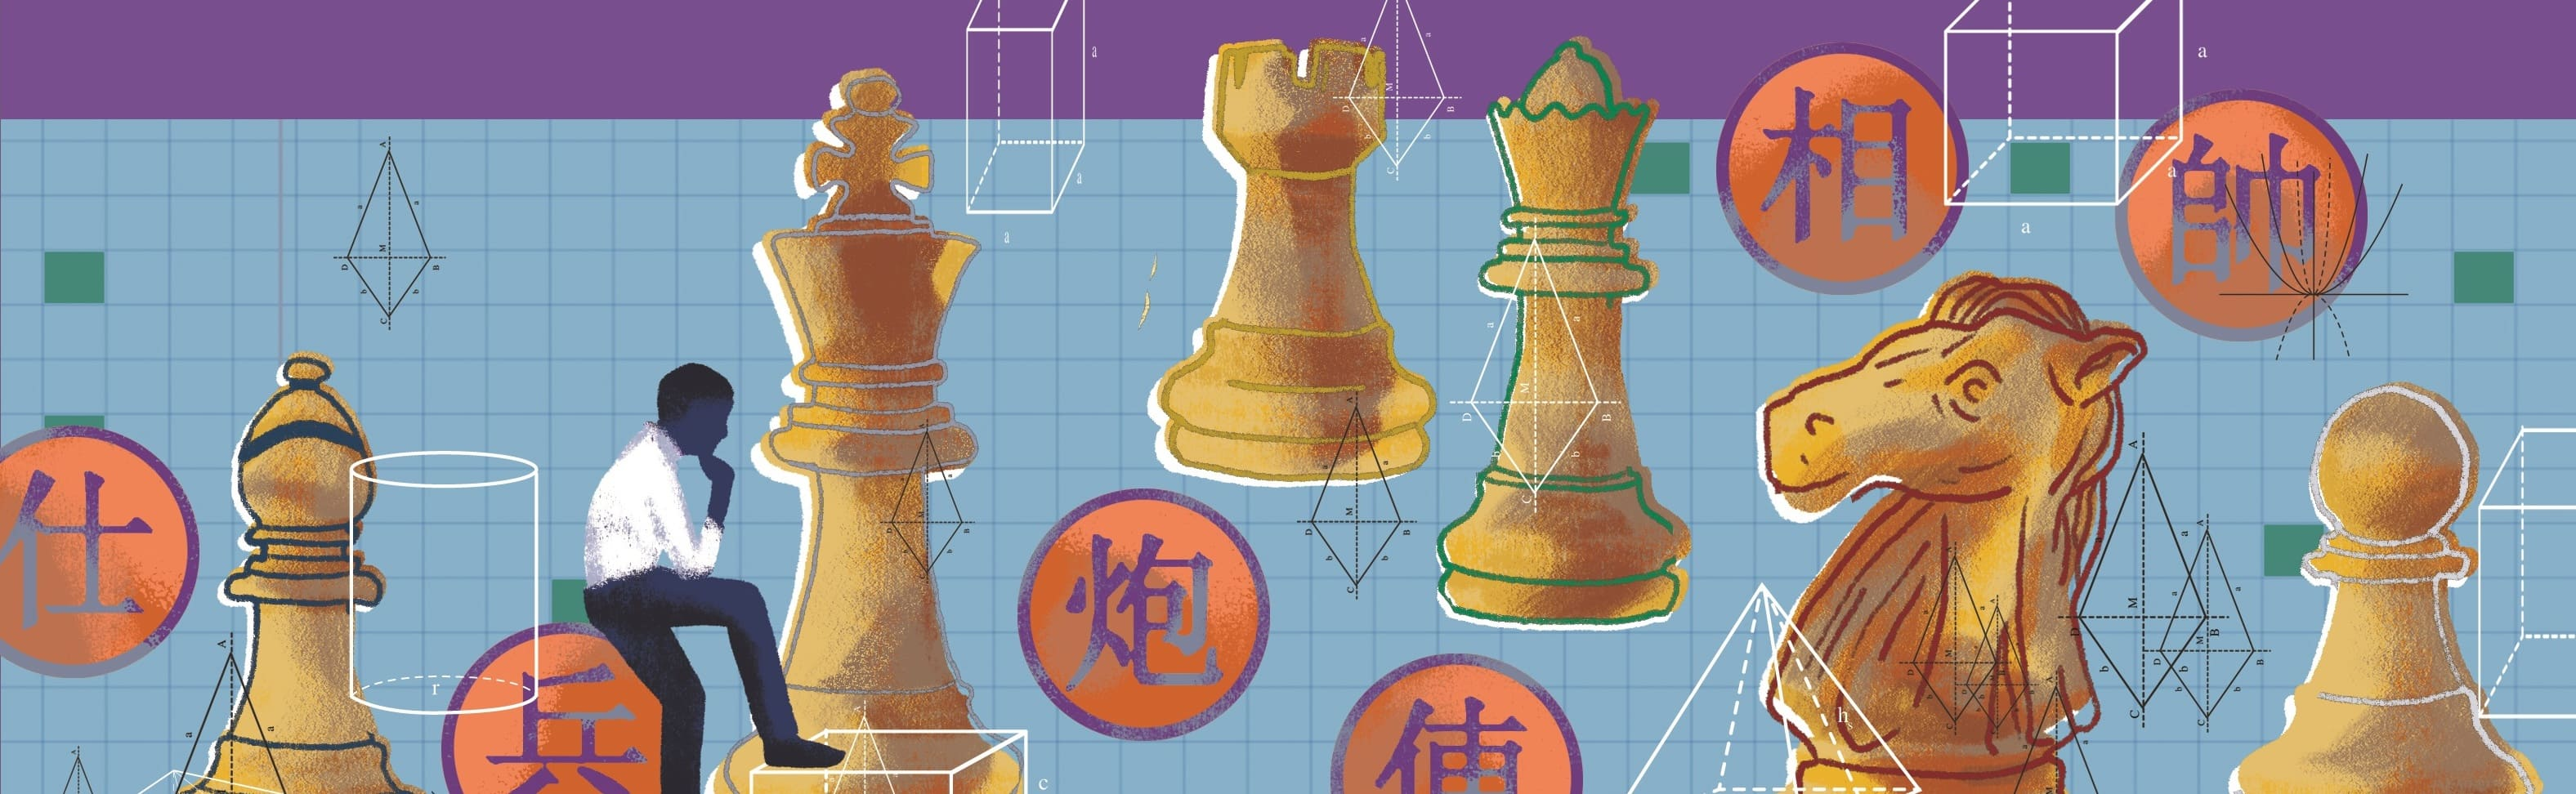
\includegraphics[width=19.3cm]{../bannergocco}}}
\AddToShipoutPicture*{\put(58,550){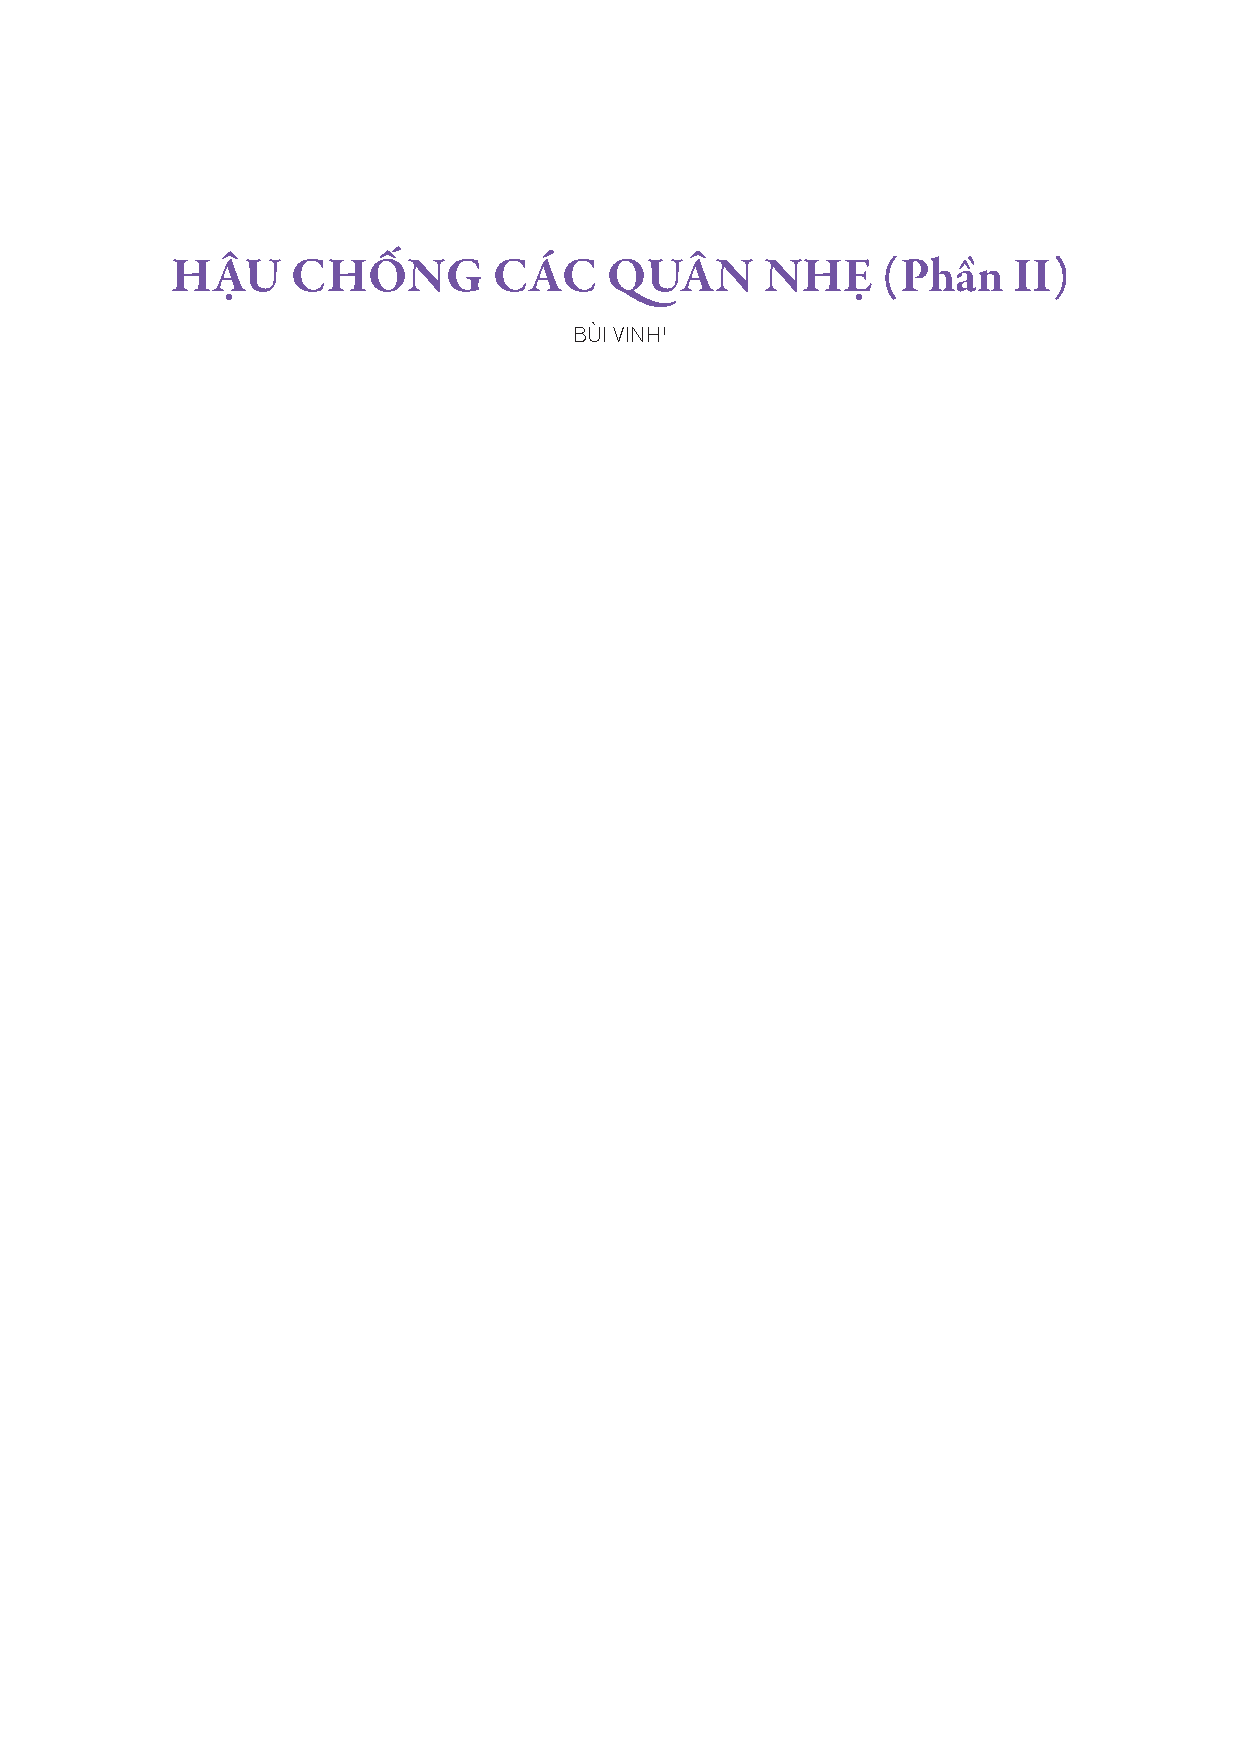
\includegraphics[scale=1]{../tieude3.pdf}}} 
\centering
\endgroup

\vspace*{155pt}

\begin{multicols}{2}
	$3.$ \textit{Hậu chống hai mã}
	\vskip 0.1cm
	Ví dụ $3$: F Dedrie
	\begin{center}
		\newgame
		\fenboard{5Q2/8/6k1/8/3n4/4K3/4n3/8 b Q - 0 1}
		\showboard
		\vskip 0.1cm
		\textit{\small\color{gocco}Hình $7$.}
	\end{center}
	Khác với cặp Tượng, Hậu chống cặp mã thường dễ dàng  giành chiến thắng. Tuy nhiên bên có Hậu cần phải thận trọng đối với các nước bắt đôi của Mã
	$\pmb{1.}$\textbf{\color{gocco}Hf$\pmb{1}$! Vg$\pmb{7}$ $\pmb{2.}$Hf$\pmb{2}$ Vg$\pmb{6}$ $\pmb{3.}$Hf$\pmb{8!}$} [Cặp mã đen đang giữ nhau khá chắc, trắng chủ động nhường nước đi để buộc đen phải di chuyển một trong hai con mã]
	\vskip 0.1cm
	$\pmb{3}$\textbf{\color{gocco}...Vg}$\pmb{5}$ [$3$...Vh$7$ $4.$Hf$6$ Vg$8$ $5.$Vf$2$ Vh$7$ $6.$Hg$5$ Vh$8$ $7.$Hg$6!$ 
	\vskip 0.1cm
	Đen bắt buộc phải di chuyển mã và tất cả các nước đi đều dẫn đến mất mã; $3$...Vh$5$ $4.$Hg$8$ Vh$6$ $5.$Vf$2$ Vh$5$ $6.$Hg$7$ Vh$4$ $7.$Hg$6$
		\begin{center}
		\newgame
		\fenboard{7k/8/6Q1/8/3n4/8/4nK2/8 b Q - 0 1}
		\showboard
		\vskip 0.1cm
		\textit{\small\color{gocco}Hình $8$.}
	\end{center}
	Đen lại không có nước đi nào tránh khỏi mất mã $7$...Vh$3$? $8.$Hh$5\#$]
	\begin{center}
		\newgame
		\fenboard{1K6/8/3n4/1n1k4/8/8/8/5Q2 b Q - 0 1}
		\showboard
		\vskip 0.1cm
		\textit{\small\color{gocco}Hình $9$.}
	\end{center}
	$\pmb{4.}$\textbf{\color{gocco}Hf$\pmb{7}$ Vh$\pmb{6}$ $\pmb{5.}$Hg$\pmb{8}$ Vh$\pmb{5}$ $\pmb{6.}$Vf$\pmb{2}$ Vh$\pmb{6}$ $\pmb{7.}$Hg$\pmb{4!}$ Vh$\pmb{7}$ $\pmb{8.}$Hg$\pmb{5}$ Vh$\pmb{8}$ $\pmb{9.}$Hg$\pmb{6}$}
	\vskip 0.1cm
	\textbf{\color{gocco}NN} $1945$,
	\vskip 0.1cm 
	Trong một vài trường hợp đặc biệt khi mà cặp Mã liên kết với nhau nếu tạo ra một hàng rào để nhốt vua đối phương trong góc, bên có Hậu sẽ không thế giành chiến thắng.
	\vskip 0.1cm
	$\pmb{1.}$\textbf{\color{gocco}Hd}$\pmb{3+}$ [$\pmb{1.}$Hf$\pmb{4}$ Vc$\pmb{5}$]
	\vskip 0.1cm
	$1$...Vc$5$ $2.$He$3+$ Vd$5$ $3.$Hg$5+$ Vd$4$ $4.$Hf$4+$ Vd$5$ $5.$Hd$2+$ Vc$5$ $6.$Hg$2$ Vc$4$
	\vskip 0.1cm
	\textbf{\color{gocco}Bài tập về nhà}
	\begin{center}
		\newgame
		\fenboard{8/8/5kn1/5b2/3K4/8/7Q/8 b Q - 0 1}
		\showboard
		\vskip 0.1cm
		\textit{\small\color{gocco}Hình $10$.}
	\end{center}
	Kế hoạch giành chiến thắng của Trắng là kiểm soát các ô mầu đen, mầu ô chỉ mã đen có thể kiểm soát.
	\vskip 0.1cm
	$\pmb{1.}$\textbf{\color{gocco}Hd$\pmb{6+}$ Vg}$\pmb{5}$ [Nếu $1$...Te$6$ $2.$Ve$4$ Vf$7$ $3.$Hd$4$ Tc$8$ $4.$Hf$2+$ Vg$7$ $5.$Vd$5$ Vh$6$ $6.$Vd$6$ Tg$4$ $7.$Hc$5$ Vh$7$ $8.$Hg$5$ Tc$8$ $9.$Hh$5+$ Vg$7$ $10.$Hc$5$ 
	\vskip 0.1cm
	Đen buộc phải di chuyển mã $10$...Tb$7$ (\textit{$10$...Ta$6$ $11.$Ha$7+$; $10$...Tg$4$ $11.$Hd$4+$; $10$...Th$3$ $11.$Hc$3+$}) $11.$Hc$7+$]
	\vskip 0.1cm
	$\pmb{2.}$\textbf{\color{gocco}Ve$\pmb{3}$!} [Trắng tìm mọi cách để bắt buộc mã đen phải di chuyển]
	\vskip 0.1cm
	$\pmb{2}$\textbf{\color{gocco}...Vg}$\pmb{4}$ [Nếu $2$...Tg$4$ $3.$Ve$4$; $2$...Tc$2$ $3.$Hc$7$ ($3.$\textit{Hd$8+$ Vg$4$ $4.$Hd$6$ Vg$5$}) $3$...Tf$5$ $4.$Hd$8+$ Vg$4$ $5.$Hf$6$ Tc$2$ (\textit{$5$...Mh$4$ $6.$Hd$4+$ Vg$5$ $7.$Hf$4+$ Vh$5$ $8.$Hh$2$ Vg$5$ $9.$Hg$3+$ Tg$4$ $10.$Hf$4+$ Vh$5$ $11.$Hf$6$ Mg$6$ $12.$Vf$2!$ Vh$6$ $13.$Vg$3$ Tc$8$ $14.$Hf$3$ Td$7$ $15.$Hd$5$ Tc$8$ $16.$Hd$3$ Tb$7$ $17.$Hd$2+$}) $6.$Hf$3+$ Vg$5$ $7.$Hg$2+$]
	\begin{center}
		\newgame
		\fenboard{2b5/6k1/3K2n1/2Q5/8/8/8/8 b Q - 0 1}
		\showboard
		\vskip 0.1cm
		\textit{\small\color{gocco}Hình $11$.}
	\end{center}
	$\pmb{3.}$\textbf{\color{gocco}Hf$\pmb{6}$ Mh}$\pmb{4}$ [$3$...Tb$1$ $4.$Hf$3+$ Vg$5$ $5.$Hg$2+$ Vf$6$ (\textit{$5$...Vh$6$ $6.$Hh$1+$}) $6.$Hb$2+$]
	\vskip 0.1cm
	$\pmb{4.}$\textbf{\color{gocco}Hd$\pmb{4+}$ Vg$\pmb{5}$ $\pmb{5.}$Hf$\pmb{4+}$ Vh$\pmb{5}$ $\pmb{6.}$Vd$\pmb{4}$ Tg$\pmb{4}$ $\pmb{7.}$Hc1} [Trắng đe dọa Ve$5-$f$6$]
	\vskip 0.1cm
	$\pmb{7}$\textbf{\color{gocco}...Mg$\pmb{6}$ $\pmb{8.}$Ve}$\pmb{4}$ [Bây giờ thì chỉ còn Tượng đen có thể di chuyển]
	\vskip 0.1cm
	$\pmb{8}$\textbf{\color{gocco}...Te}$\pmb{6}$ [Các phương án khác cũng không tốt cho đen $8$...Td$7$ $9.$Hd$1+$ Tg$4$ $10.$Hd$2$ Te$6$ $11.$Hd$6$ Th$3$ $12.$Hc$5+$ Vh$4$ $13.$He$3$ Đen rất kho tránh khỏi mất quân $13$...Vg$4$ $14.$He$2+$ Vh$4$ Đen cố gắng phối hơp giữa tượng và mã để tạo ra hàng rào ngăn vua trắng tiếp cận gần với vua đen. Tuy nhiên, đen khó tránh khỏi mất quân $15.$Hd$2$ Tg$4$ $16.$Hh$6+$ Th$5$ $17.$Vf$5$ Me$7+$ $18.$Ve$5$ Mg$6+$ $19.$Vf$6+–$; $8$...Mh$4$ $9.$Ve$5$; $8$...Vh$4$ $9.$Hh$6+$ Th$5$ $10.$Vf$5$ Me$7+$ $11.$Ve$6$ Mg$6$ $12.$Vf$6$]
	\vskip 0.1cm
	$\pmb{9.}$\textbf{\color{gocco}Hd$\pmb{2}$ Th$\pmb{3}$ $\pmb{10.}$Hh$\pmb{2}$ Vg$\pmb{4}$ $\pmb{11.}$Ve$\pmb{3!}$} 
	Đen lại bị ``xung xoang"]
	\vskip 0.1cm
	$\pmb{11}$\textbf{\color{gocco}...Mh$\pmb{4}$ $\pmb{12.}$Hg$\pmb{1+}$ Tg$\pmb{2}$ $\pmb{13.}$Vf$\pmb{2}$ Vh$\pmb{3}$ $\pmb{14.}$Hb$\pmb{1}$! Tf$\pmb{3}$ $\pmb{15.}$Hb}$\pmb{8}$ [Trắng dọa chiếu hết ở g$3$]
	\vskip 0.1cm
	$\pmb{15}$\textbf{\color{gocco}...Vg$\pmb{4}$ $\pmb{16.}$Hb$\pmb{4+}$ Vh}$\pmb{5}$ [$16$...Vh$3$ $17.$Hf$4$]
	\vskip 0.1cm
	$\pmb{17.}$\textbf{\color{gocco}Vg$\pmb{3}$!}
	\begin{center}
		\newgame
		\fenboard{8/8/8/7k/1Q5n/5bK1/8/8 b Q - 0 1}
		\showboard
		\vskip 0.1cm
		\textit{\small\color{gocco}Hình $12$.}
		\end{center}
	\vskip 0.1cm
	\columnbreak
	Đen mất quân và thua cờ.
	\vskip 0.1cm
	$\pmb{1-0}$
\end{multicols}